\chapter{Experiments}%
\label{ch:experiments}
As we have laid out in the previous chapter our method mainly depends on the quality of the learned source priors. The generative prior models have to provide an exhaustive and exclusive approximation of the data manifold or its data source. Therefore our experiments strongly focus on analyzing the prior densities under different training regimes and inputs. In general, we have two separate datasets with which we run the experiment, as described in the following section. For each experiment, we use two different data representations. First using the raw time-domain data and second a mel-spectrogram transformation into frequency space. As explained in \cref{ch:background} the frequency representation is lacking phase information which would necessitate a vocoder model to invert the destructive frequency transformation. We keep this step out of scope for this work, as there are also separate successful works on reversing spectrograms to time-domain~\cite{something about vocoders}.


\section{Datasets}
We will be working on two datasets. First, a simplified Toy dataset which reduces the problem to a minimal canonical one and second the \texttt{musdb18} dataset which is a widely-used test-set for musical source separation.

We fix the sampling rate of both datasets to \(16.000 \si{\Hz}\).
For both the Toy Data and the \texttt{musdb18} dataset we experiment with prior models on time-domain and spectral-domain input.

\subsection{ToyData}
\begin{marginfigure}[5em]
    \resizebox{\textwidth}{!}{%
        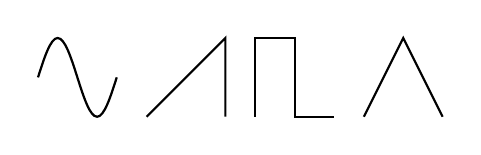
\begin{tikzpicture}
    \node[matrix,thick,column sep=1em,row sep=1em]
    {
        \draw (0,0.5) sin (0.25,1) cos (0.5,0.5) sin (0.75,0) cos (1,0.5); &
        \draw (0,0) -- (1,1) -- (1,0); &
        \draw (0,0) -- (0,1) -- (0.5,1) -- (0.5,0) -- (1,0); &
        \draw (0,0) -- (0.5,1) -- (1,0); \\
    };
\end{tikzpicture}
%
    }%
    \caption{One period of each of the four toy sources: sinus, sawtooth, square and triangle wave.}%
    \label{fig:toy_data}
\end{marginfigure}

We simplify the problem domain to create a toy-like dataset. We randomly generate waves from four simple oscillations, see~\cref{fig:toy_data}. Given a wave from each source, the mix is computed by simply taking the mean. When sampling from each source we randomly select a period and phase. The frequencies are restricted to the frequency bounds of the 88 keys of an equal-temperament tuned piano. In our experiments we are gonna model these sources with probability densities, looking especially at the square that will pose a problem, as those only consist of two unique values (\(-1\) and \(1\)). This collapsing posterior would simplify the problem too much, therefore we also vary the amplitude of the sampled signals in the uniform range \([0.8, 1.0]\).

In ++later++ section we show that estimating densities over these waves is not giving a smooth manifold. Or differently: in the latent space we can not interpolate between two signals, because the model models, simply put, the sample waves as spiked Dirac deltas.


\subsection{musdb18}
Further we use the \texttt{musdb18}~\cite{rafiiMUSDB182017} dataset published for the 2018 Signal Separation Evaluation Campaign~\cite{stoter20182018}. The dataset consists of 150 full songs covering various artists and genres, split into train and test sets sized 100 and 50, respectively. Each track is separated into the four sources \emph{drums}, \emph{bass}, \emph{vocals} and \emph{others}. The \emph{others} source channel contains any remaining set of instruments not categorized under the first three ones. The song files are provided in the Stem audio file format~\cite{nativeinstrumentsStem} and encoded at 44.1kHz. Stem here is terming the provided source channels, we use the terms interchangeably.

The dataset consists of the 100 tracks taken from the DSD100~\cite{SiSEC16} dataset and 46 track out of the MedleyDB~\cite{bittnerMedleyDB2016} dataset. Both dataset contain tracks from a wide range of (western) musical genres, Rock, Pop, Rap, Jazz and Metal. While the upstream data sources provide more fine-grained meta-data, \texttt{musdb18} brings all tracks into the same format and stem splitting as described above.

Next to the separated stems, the dataset provides the original (studio) mix for each song. This mix is not equivalent to the simple linear mixing which we get by taking the mean. Nevertheless, the provided mix diverges only insignificantly from an auto-generated mix, as the original sources are provided in their post-compression, post-mixed form. This means that we can use the original mix and assume it to be reasonably close to the canonical linear mix.

As the songs are real natural songs, they are of different lengths. Our models will, in difference, to many other recent methods, not be auto-regressive. Thus we sample fixed-length cuts from the songs as training and test samples. For the \texttt{musdb18} data, no pre-processing is applied, as the data already contains the wanted level variability, it spanning different genres and artists.

It is noted that the \texttt{musdb18} dataset while providing a remarkable diverse 10hr of real-world music, is a rather small numbered set of samples. Any data modelling from this set of data will consequently be biased. The dataset specifically is created for the accompanying separation challenge and will not translate to general music modelling.

\section{Prior architectures}
\begin{table}
    \begin{tabular}{rccccc}
                                & blocks & flows & layers & kernel size & features\\\midrule
        toy (time)              & 4      & 6     & 10     & 3           & 32      \\
        \texttt{musdb18} (time) & 8      & 6     & 10     & 3           & 48      \\
        toy (mel)               & -      & -     & -      & -           & -       \\
        \texttt{musdb18} (mel)  & 4      & 32    & 3      & 3           & 512     \\
    \end{tabular}%
    \caption{The network architectures for the four prior models.}%
    \label{tab:priors}%
\end{table}

We construct four distinct prior models for the two datasets and input data representations, respectively. All models follow the flow architecture described in \sref{ch:method}. \cref{tab:priors} gives a summary of the networks. Remember for the time-domain priors the affine transformations are parametrized by WaveNets, consisting of multiple one-dimensional convolutions. For the spectrogram priors, each is parametrized by un-dilated two-dimensional convolutions as described before. Because the complexity of the coupling layer is smaller in this case, we increase the number of flows per block~\cite{kingmaGlow2018}. In both cases the last layer is initalized to zero, reducing each affine coupling layer to the identity at the beginning of training. The number of features in each convolutional layer is fixed throughout the whole network, as given in the table. All kernels are size \(3\) or \(3\×3\), respectively.

\section{Training the priors}
Training of the priors is done in mini-batches with an Adam optimizer~\cite{kingmaAdam2017}. The initial learning rate is set to \(1e-4\). The learning rate is decreased with \(γ=0.6\) and a fixed five step decrease schedule.

% \begin{figure}
%     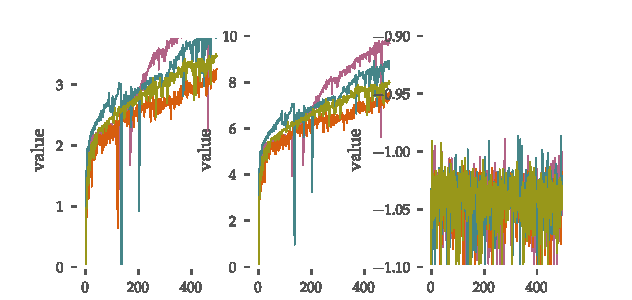
\includegraphics{toy_training_curves.pdf}
%     \caption{The training curves of the toy data curves}
% \end{figure}

We fine-tune the noise-less flow models by continuing the training with added Gaussian noise on the input samples. Fine-tuning~\cite{yosinskiHow2014} the noise-conditioned model instead of retraining the model is considerably cheaper and the noised distribution we want to approximate is close to the noise-free distribution of the initial training. We find that fine-tuning converges quickly at ----. We

\section{Testing the priors}
Training of the normalizing flow model combines the two objectives: First, we maximize the log-determinant of the \I{non-volume preserving} affine coupling and the activation normalization layers. This guarantees us the invertibility of these transformations. Second, we maximize the likelihood of the projected samples under the chosen target distribution~\footnote{The target distribution is the prior to our prior model. It is set to a factorized Gaussian.}. For the evaluation, we are interested in the mean average likelihood under the target distribution for different in- and out-of-distribution inputs. Remember that the flow gives a bijective mapping between the input and target space~\footnote{necessitated by the invertibility}. For an input of size \(\x \∈ \ℝ^{1\×L}\) the flow returns a latent \(\z \∈ \ℝ^{1\×L}\) of the same size. Each time-point latent \(\z_t\) depends on the  inputs from the receptive field of the flow before and after the respective input \(\x_t\) but is evaluated under the independent margin \(\z_t \sim \N(0,1)\). Because therefore the factorized multivariate Gaussian prior is equivalent to a set of one-dimensional Gaussians, the flow is also not size restricted. All transformations in the network are convolutional and use appropriate padding. \(L\) can be any chosen length. We want to set the input length larger than the receptive field of the network. The latents on either end side of the sample will be based on the larger amount of padded input, while the center values from the sample receive the full receptive field. The size of the receptive field is regimented by the depth and kernel sizes used in the convolutions of the coupling layers and the number of squeeze operations in the blocks (see \cref{fig:squeeze}). For an exact derivation of the receptive field size see {\color{red}Appendix recp size}.

We show an example of sampling from the toy data priors in time-domain in \cref{fig:toy_time_sample}. It should be unsuprising that the drawn samples are not returning a consistent curve. Each independent latent is connected to a local output defined by the recpetive field. As all latents are i.i.d. the generative process, generates locally consistent curves.

% \begin{figure}
%     \includegraphics{toy_samples_time.pdf}%
%     \label{fig:toy_time_sample}%
%     \caption{Samples from the time-domain prior trained on the toy data.}
% \end{figure}

\subsection{De-noising}
% \begin{marginfigure}
%     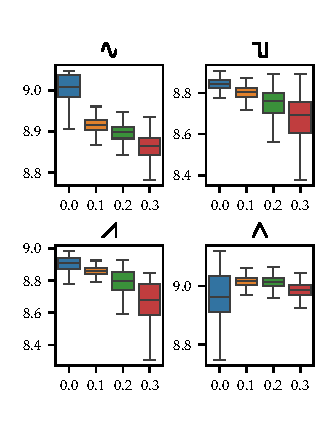
\includegraphics{noise_likelihood_with_noise}%
%     \caption{noise likelihood with noise}%
%     \label{fig:noise_ll_with_noise}
% \end{marginfigure}

De-noising is the

In this ablation study we want to check how resilient the generative prior models are to noisy samples. It is hypothesized that the latent space of the model consists of, intuitively, singular peaks at mappings of in-distribution samples~\cite{jayaramSource2020}. For the separation to be able to optimize under the prior density, we need likelihood to slowly decrease when moving away from positive samples. If the distribution is too peaked only noiseless inputs would be highly likely and adding noise quickly makes samples too unlikely. We propose adding Gaussian noise with a random variance to the positive samples during training. This should smooth out the modeled density.

% \begin{marginfigure}
%     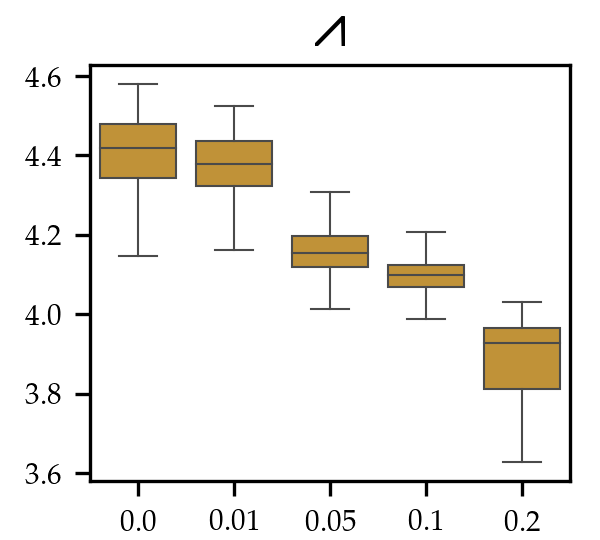
\includegraphics{noise_likelihood_without_noise}%
%     \caption{noise likelihood without noise}%
%     \label{fig:noise_ll_without_noise}
% \end{marginfigure}

\subsection{Testing cross-likelihood}
In the full model each prior is used to extract its source channel separately. Through their training they explicitly contract the density for the positive, in-class examples. During separation the priors therefore encounter negative, out-of-distribution samples for the first time. To be useful for separation, it is important that the priors give a low likelihood to samples from the other classes of the dataset.

% \begin{marginfigure}
%     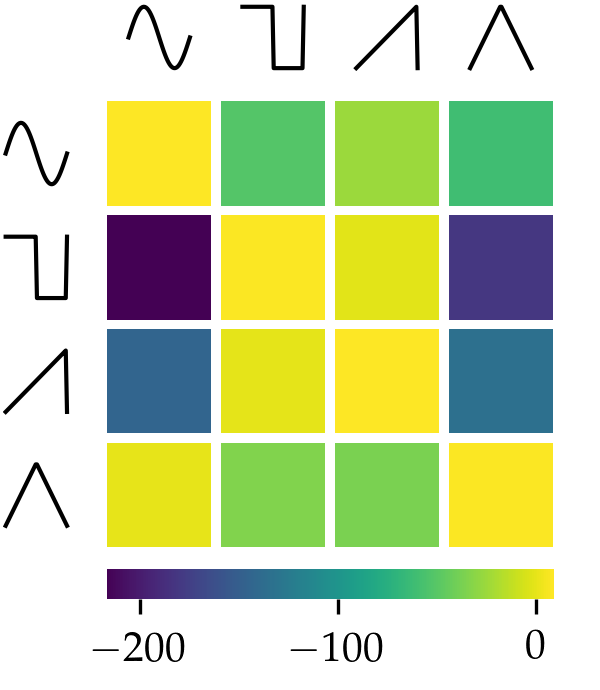
\includegraphics{heatmap_toy}%
%     \caption{We display the mean average log likelihood of the test data under the different priors and the different signal sources.}%
%     \label{fig:heatmap_toy}
% \end{marginfigure}

We test for this by calculating the mean log likelihood of the the test data set under each prior, for each source channel separately. What we anticipate is that the samples from the priors training source are of high likelihood while all other sources are low likelihood. In \cref{fig:heatmap_toy} we show the source dependent likelihoods for the Toy Data. The in-distribution samples are all of high likelihood while all out-of distribution samples are highly un-likely. The Flow model therefore was able to detect out-of-distribution samples while only being trained on in-distribution samples~\footnote{Something psychological research has shown, humans being able to do.}. The estimated densities are discriminative.

When running the same experiment for the musdb18 the discriminative power does not hold up, see~\cref{fig:heatmap_musdb}. All signal sources are about equally likely under each prior density. We hypothesize this stems from the fact that the real musical data is severely more complicated compared to the Toy Data. The Flows model the appearance of sound in general, as the in-class variability of sounds is already high, without knowing anything about the \I{discriminative} differences between the instruments and does not infer the distribution from those features.

% \begin{marginfigure}
%     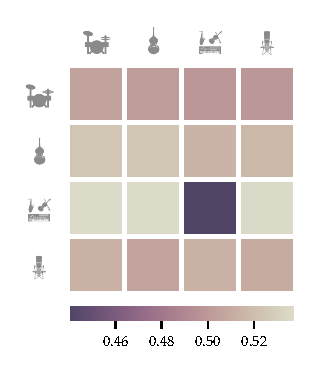
\includegraphics{heatmap_musdb}%
%     \caption{We display the mean average likelihood of the test data under the different priors and the different signal sources.}%
%     \label{fig:heatmap_musdb}
% \end{marginfigure}

Even above that the results exhibit an additional failing for the musdb18 dataset. The third stem in the dataset files \I{other} is filled with a smorgasbord of different instruments. With our training regime we are implying we can model the sound this set of unrelated instruments with only in-distribution samples with a resulting distribution which is discriminative against another set of unrelated instruments. Intuitively this already fails to be reasonable. Because of this the results show the unintuitive result that the test samples from the \I{other} class are \I{less likely} under its own prior model compared to the out-of-distribution samples. While this makes it rather final that the at hand dataset is not completely suitable to out trainings regime, it is a data-dependent restriction that would not correspond to our hypothesized application.

Similar results were shown before in~\itodo{cite some OOD VAE stuff}.

The results for both datasets are similar for all tested model architectures and input domains. See Appendix~\itodo{add results} for the full results.

\subsection{Increasing discriminative power}
With the prior models being not discriminative, it is not possible to train the separation model. Following we will try extend the priors to increase their discriminative power. Above that we propose that our method still holds merit given these results, further work on generative models might result in more discriminative generative models. The method can use any density as a drop-in replacement for the prior in the separation model.

As layed out in~\ref{ch:background} the bad out-of-distribution detection of generative models is not a surprising result and multiple recent works go about solving this. We want to increase the

% \begin{marginfigure}
%     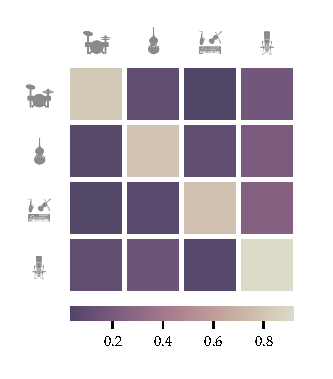
\includegraphics{heatmap_musdb_classifier}
%     \caption{The logits of different classes of the different outputs}%
%     \label{fig:heatmap_musdb_classifier}
% \end{marginfigure}

\section{Testing the posteriors}

\subsection{TODO EXPERIMENTS}
\begin{enumerate}
    \item Adding noise ⇒ better likelihood
    \item De-noising single signals
\end{enumerate}
